\begin{samplecase}
{\bf Different optical models : n + ${}^{120}$Sn}\newline
To demonstrate the variety of optical models that we have added to 
TALYS, we include a sample case in which 4 OMP's for neutrons on 
$^{120}$Sn are compared. The results are given in Fig. \ref{sntotal} for
the total cross section and in Fig.\ref{sninl} for the total inelastic cross 
section.
\subsubsection{Case a: Koning-Delaroche local potential}
The input file is

\VerbatimInput{\samples n-Sn120-omp-KD03/org/talys.inp}

This is the default calculation: TALYS will find a local OMP in the 
structure database and will use it.
\subsubsection{Case b: Koning-Delaroche global potential}
The input file is

\VerbatimInput{\samples n-Sn120-omp-KD03global/org/talys.inp}

\subsubsection{Case c: Koning-Delaroche local dispersive potential}
The input file is

\VerbatimInput{\samples n-Sn120-omp-KD03disp/org/talys.inp}

\subsubsection{Case d: Bauge-Delaroche JLM potential}
The input file is

\VerbatimInput{\samples n-Sn120-omp-jlm/org/talys.inp}

\end{samplecase}
\begin{figure}
\centering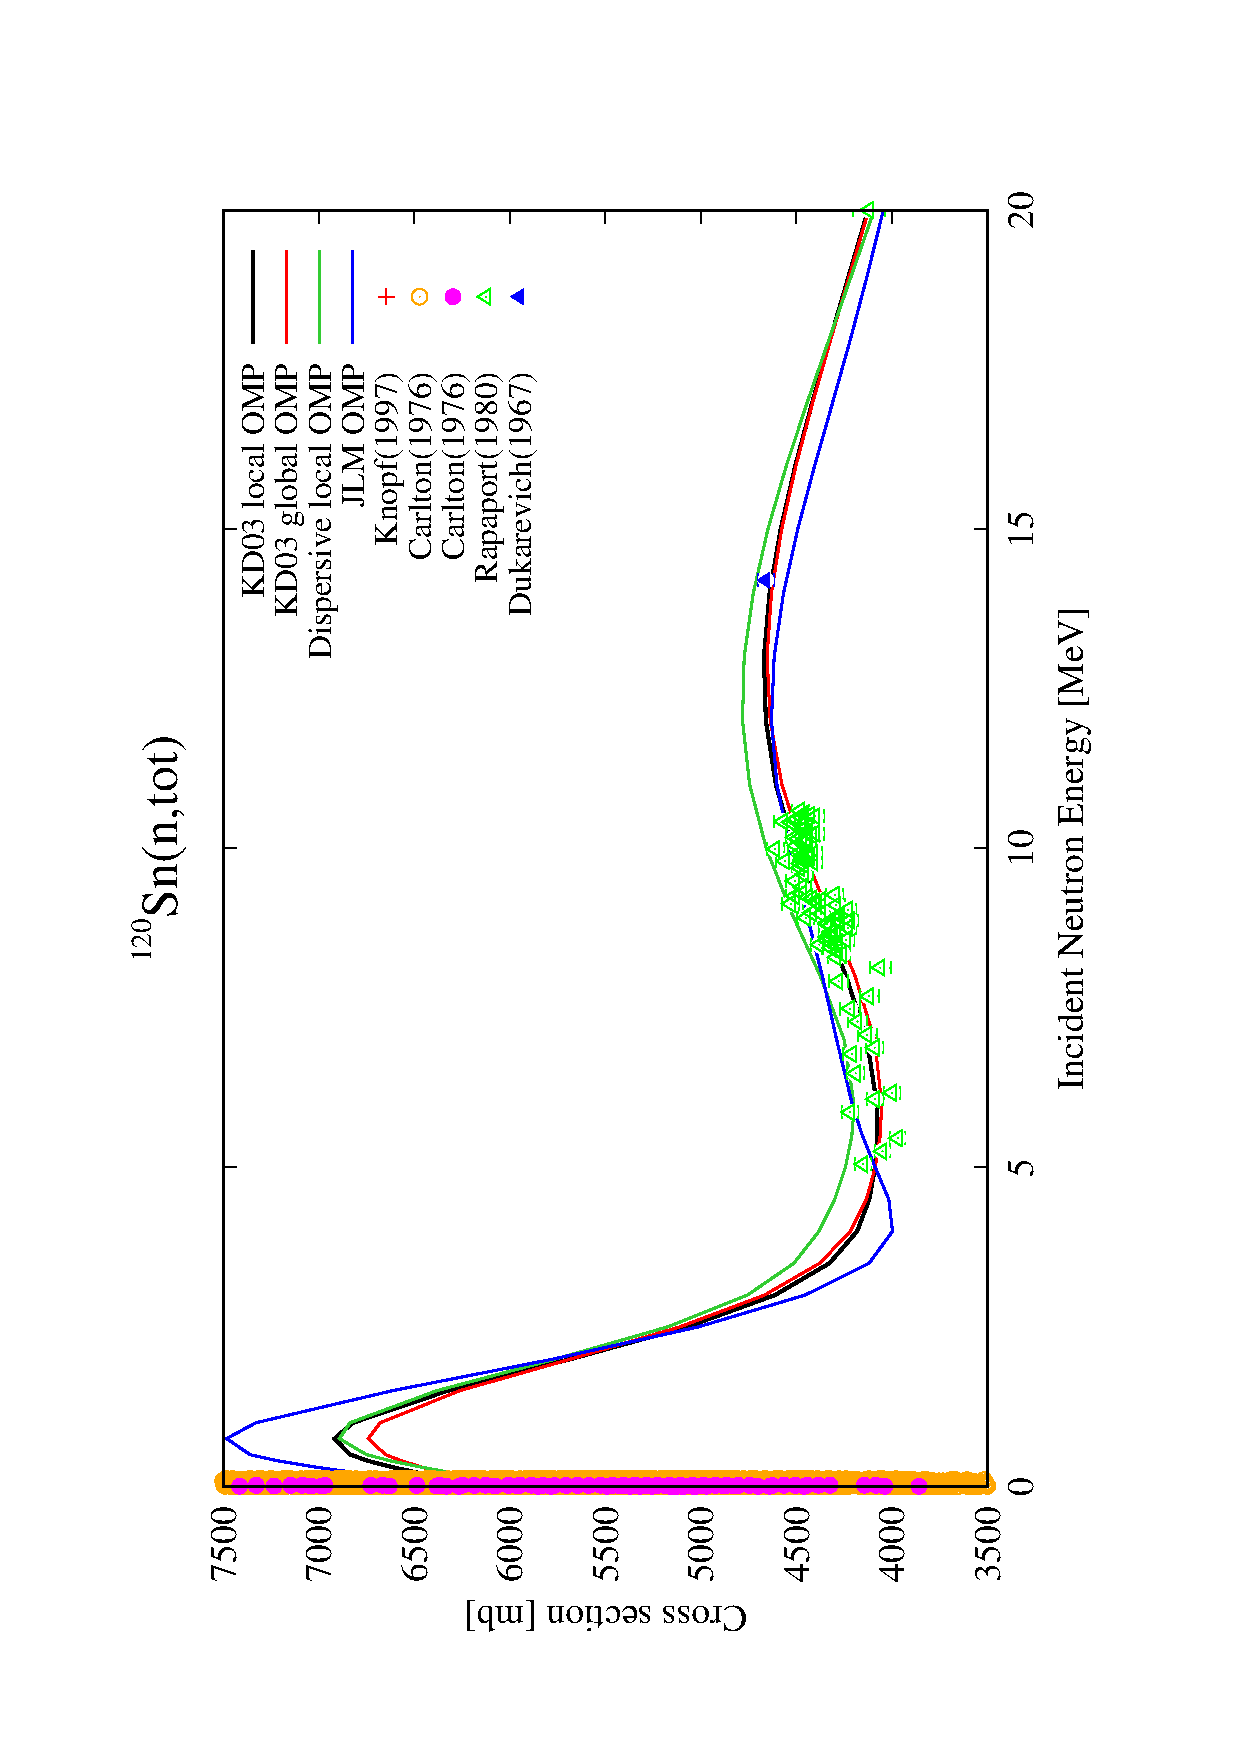
\includegraphics[scale=0.5,angle=270]{n-Sn120-omp}
\caption{Total cross section for neutrons incident on $^{120}$Sn for
different optical model potentials.}
\label{sntotal}
\end{figure}
\begin{figure}
\centering\includegraphics[scale=0.5,angle=270]{n-Sn120-inel}
\caption{Total inelastic cross section for neutrons incident on $^{120}$Sn for
different optical model potentials.}
\label{sninl}
\end{figure}
